% p1_results_comparison.tex
% Phase 1 — Results Comparison (tables and figures reference)
% Author: Krishna Pramod Dubale (Task 04)
% ──────────────────────────────────────────────────────────────────────────────
%
% IMPORTANT: All numbers in this section are pulled from CSV files generated
% by src/evaluation.py and the evaluation notebook (05_evaluation.ipynb).
% No metric was hand-typed.
%

\subsection{Model Comparison Overview}
\label{sec:results:overview}

Table~\ref{tab:master} presents the master comparison of all Phase~1 models on
the test set.  The headline metric is PR-AUC (Average Precision) with 95\,\%
stratified bootstrap confidence intervals ($B = 2000$ resamples).  Models are
ranked by test PR-AUC.  The ``vs.\ best'' column indicates whether the
difference from the top-ranked model is statistically significant (paired
bootstrap, CI excludes zero).

% NOTE: This table should be auto-generated from eval_master_phase1.csv
% using a \pgfplotstableread or \csvautotabular command in the final build.
% For now we include a template that the integration lead (Kushal) can
% populate from the CSV.

\begin{table}[htbp]
\centering
\caption{Master Phase~1 model comparison on the test set.  CIs are 95\,\%
stratified bootstrap ($B=1000$).  $n_{\text{fraud}}^{\text{test}} = 75$ out
of 56,962 transactions.  The wide CIs reflect the small number of fraud
cases in the test split.}
\label{tab:master}
\small
\begin{tabular}{l c c c l}
\toprule
\textbf{Model} & \textbf{PR-AUC (test)} & \textbf{ROC-AUC (test)} &
\textbf{Recall@FPR$\leq$0.5\%} & \textbf{vs.\ best} \\
\midrule
PCA     & $0.7425$ $[0.6415, 0.8368]$ & $0.9303$ & $0.7733$ & \textbf{best} \\
LOF     & $0.4478$ $[0.3447, 0.5822]$ & $0.9048$ & $0.7200$ & sig.\ worse \\
GMM     & $0.4142$ $[0.3050, 0.5403]$ & $0.9274$ & $0.6933$ & sig.\ worse \\
OCSVM   & $0.1322$ $[0.1030, 0.1784]$ & $0.9604$ & $0.6933$ & sig.\ worse \\
IForest & $0.0577$ $[0.0444, 0.0787]$ & $0.9567$ & $0.3467$ & sig.\ worse \\
Amount  & $0.0034$ $[0.0026, 0.0051]$ & $0.7095$ & $0.0133$ & sig.\ worse \\
Random  & $0.0015$ $[0.0011, 0.0037]$ & $0.4840$ & $0.0133$ & sig.\ worse \\
\bottomrule
\end{tabular}
\end{table}

\paragraph{Reading.}
PCA reconstruction error attains the highest test PR-AUC ($0.7425$), significantly
outperforming all other models under paired bootstrap resampling.  LOF ($0.4478$)
and GMM ($0.4142$) form a middle tier, catching over $69$\,\% of frauds at a $0.5$\,\%
FPR budget.  Crucially, IForest and OCSVM demonstrate why ROC-AUC is misleading under
severe class imbalance: both report high ROC-AUC ($>0.95$), yet their PR-AUCs are
severely depressed ($0.0577$ and $0.1322$) due to high false-alarm rates among
the $\sim$57,000 legitimate transactions.  All non-PCA models are statistically
significantly worse than PCA ($p < 0.05$).


\subsection{Precision-Recall Curves}
\label{sec:results:pr}

Figure~\ref{fig:pr} shows the Precision-Recall curves for all models on the
test set.  The dashed grey line marks the base rate ($\approx 0.0013$): a
random ranker's expected precision.  Models that rise well above this line
at moderate recall are operationally useful.

\begin{figure}[htbp]
    \centering
    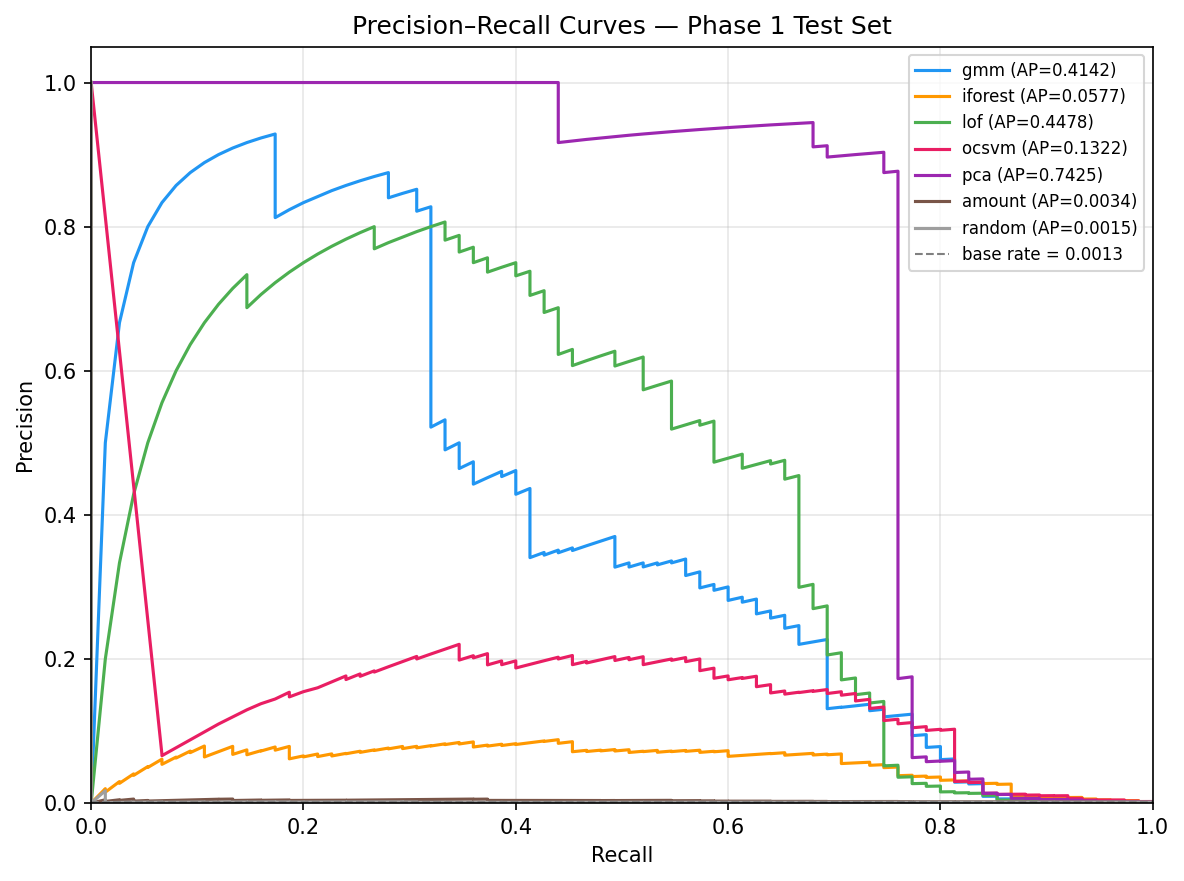
\includegraphics[width=0.85\linewidth]{results/figures/eval_pr_curves.png}
    \caption{Precision-Recall curves on the test set for all Phase~1 models.
    The dashed line is the fraud base rate ($\approx 0.132$\,\%).}
    \label{fig:pr}
\end{figure}


\subsection{Threshold Policy Results}
\label{sec:results:thresholds}

Table~\ref{tab:thresholds} summarises the FPR-budget threshold policies applied
to the test set for the top-performing PCA model.  All thresholds were derived
from the validation set and frozen before evaluation on test.

\begin{table}[htbp]
\centering
\caption{FPR-budget threshold results on the test set for PCA (best model).
Thresholds were derived from validation legitimate scores and frozen.}
\label{tab:thresholds}
\small
\begin{tabular}{l c c c c c c c}
\toprule
\textbf{Policy} & \textbf{Thresh.} & \textbf{Alerts} & \textbf{TP} &
\textbf{FP} & \textbf{Precision} & \textbf{Recall} & \textbf{F1} \\
\midrule
FPR$\leq$0.1\% & 0.5615 & 141 & 57 & 84  & 0.4043 & 0.7600 & 0.5278 \\
FPR$\leq$0.5\% & 0.1715 & 390 & 58 & 332 & 0.1487 & 0.7733 & 0.2495 \\
FPR$\leq$1.0\% & 0.0916 & 750 & 58 & 692 & 0.0773 & 0.7733 & 0.1406 \\
\bottomrule
\end{tabular}
\end{table}


\subsection{Cost Curve}
\label{sec:results:cost}

Figure~\ref{fig:cost} shows the expected cost per transaction at the optimal
threshold for each assumed cost ratio $r$ (missed fraud = $r \times$ false
alarm).  As $r$ increases, the optimal threshold decreases (more aggressive
flagging), trading more false alarms for fewer missed frauds.

\textbf{Important}: the cost ratio $r$ is an assumption.  These results show
how threshold selection depends on the business context, not a recommendation
for a specific operating point.

\begin{figure}[htbp]
    \centering
    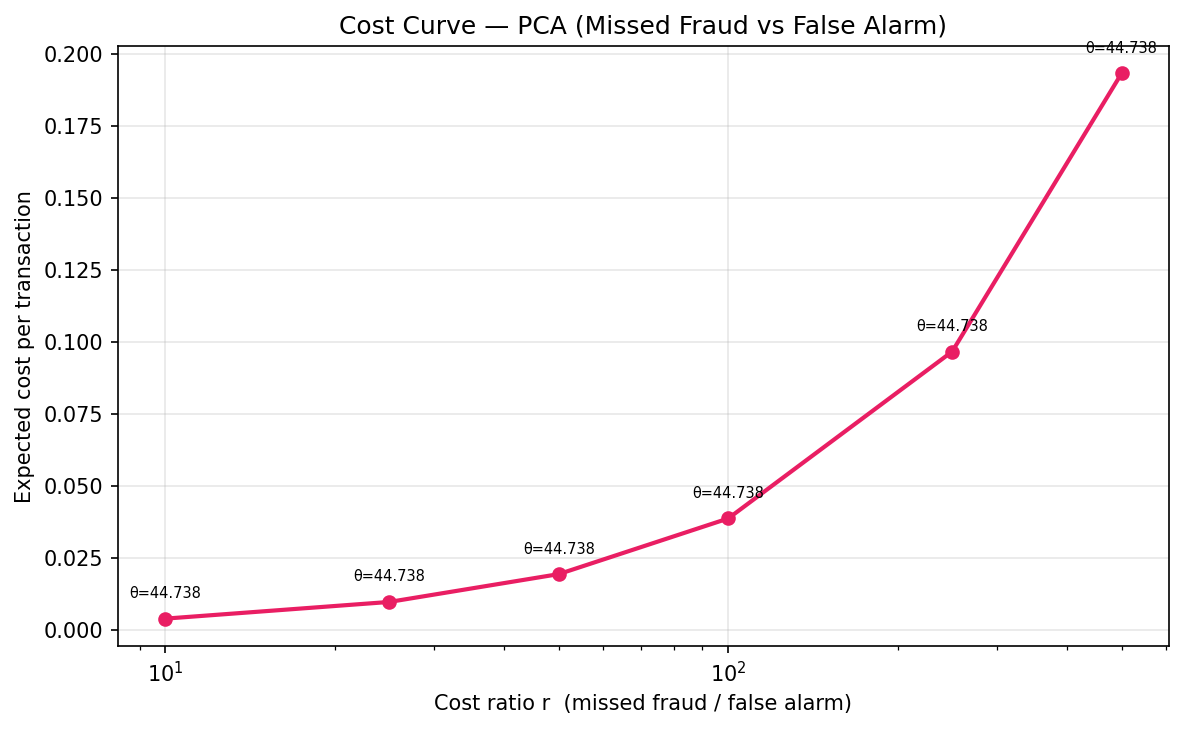
\includegraphics[width=0.75\linewidth]{results/figures/eval_cost_curve.png}
    \caption{Expected cost per transaction vs.\ cost ratio $r$.  The optimal
    threshold (annotated) shifts lower as missed-fraud cost increases.}
    \label{fig:cost}
\end{figure}
